\documentclass[11pt,oneside]{book}
\usepackage[utf8]{inputenc} 
\usepackage[T1]{fontenc} % fonts to encode unicode
\usepackage{draftflag}
\usepackage{times}
\usepackage{fullpage}
\usepackage{makeidx}
\newcounter{DOIcounter}

\makeindex
\renewcommand{\indexname}{Author Index}

\usepackage{pdfpages}   % can also use [draft] option
\usepackage[colorlinks,
%%% EDIT TITLE: %%%%%%%%%%%%%%%%%%%%%%%%%%%%%%%%%%%%%%%%%%%%%%%%%%%%
            pdftitle={Proceedings of the Workshop on IndoNLP: Proceedings of the 1st Workshop on Natural Language Processing for Indo-Aryan and Dravidian Languages @COLING-2024}, 
            pdfauthor={Association for Computational Linguistics},
            %pdfsubject={...},
            %pdfkeywords={...}
           ]{hyperref}   % hyperlinked table of contents, etc.
\hypersetup{pdfpagemode=none}
\hypersetup{plainpages=false,colorlinks=true}  % point to papers, not preface

% for A4 size %%%%%%%%%%%%%%%%%%%%%%%%%%%%%%%%%%%%%%%%%%%%%%%%%%%
\setlength{\paperwidth}{21cm}   % A4
\setlength{\paperheight}{29.7cm}% A4
\special{papersize=21cm, 29.7cm}
\pdfpageheight\paperheight
\pdfpagewidth\paperwidth
\setlength\topmargin{-5mm} \setlength\oddsidemargin{-0cm}
\setlength\textheight{24.7cm} \setlength\textwidth{16cm}
\setlength\columnsep{0.6cm}  \newlength\titlebox \setlength\titlebox{2.00in}
\setlength\headheight{5pt}   \setlength\headsep{0pt}
\setlength\footskip{0.8cm}
\setlength\leftmargin{0.0in}
\pagestyle{plain}
%%%%%%%%%%%%%%%%%%%%%%%%%%%%%%%%%%%%%%%%%%%%%%%%%%%


\usepackage{color}
\definecolor{brown}{rgb}{0.59, 0.29, 0.0}
\newcommand{\changeurlcolor}[1]{\hypersetup{urlcolor=#1}}       
\newcommand{\citeinfo}[2]{
  \AddToShipoutPicture{
    \setlength{\unitlength}{1mm}
%%%% Edit event name, dates, location and copyright (if needed)  %%%%%%%%%%%%%%%%%%%%%%
    \put(105,13){\makebox(0,0){\footnotesize {\em  Proceedings of the First Workshop on Natural Language Processing for Indo-Aryan and Dravidian Languages (IndoNLP2025)},
	\ifthenelse{\equal{#1}{#2}}{page #1}{pages #1--#2}}}
     \put(105,10){\makebox(0,0){\footnotesize January 20, 2025. \copyright 2025 Association for Computational Linguistics
}}

%%%% DO NOT USE this DOI mechanism if the proceedings will end in the ACL Anthology.
%%%% The Anthology creates their own DOIs.
%%%% DO NOT USE
%\put(105,6){\makebox(0,0){\footnotesize
%\stepcounter{DOIcounter}\urlstyle{rm}
%\url{https://doi.org/10.26615/978-954-452-056-4_\ifnum\value{DOIcounter}<10 00\else \ifnum\value{DOIcounter}<100 0\fi\fi\arabic{DOIcounter}}}}
%%%%%%%%%%%%%%%%%%%%%%%%%%%%%%%%%%%%%%%%%%%%%%%%%%%%%%%%

}}

% for A4 size %%%%%%%%%%%%%%%%%%%%%%%%%%%%%%%%%%%%%%%%%%%%%%%%%%%

\newcommand{\draftframe}[1][0]{
  \AddToShipoutPicture{
    \setlength{\unitlength}{1mm}
    \put(20,25){\line(1,0){175}}
    \put(20,276){\line(1,0){175}}
    \multiput(20,256)(0,10){4}{\line(1,0){40}}
    \multiput(20,256)(0,5){8}{\line(1,0){30}}
    \multiput(20,256)(0,1){35}{\line(1,0){20}}
    \put(70,256){\makebox(0,0){20mm}}
    \put(70,266){\makebox(0,0){10mm}}
    \put(70,286){\makebox(0,0){-10mm}}

    \put(25,20){\line(0,1){271}}
    \put(186,20){\line(0,1){271}}

    \multiput(15,172)(10,0){3}{\line(0,1){53}}
    \multiput(15,172)(5,0){5}{\line(0,1){46}}
    \multiput(15,172)(1,0){20}{\line(0,1){40}}

    \put(15,232){\makebox(0,0){-10}}
    \put(35,232){\makebox(0,0){10}}
    \put(15,227){\makebox(0,0){mm}}
    \put(35,227){\makebox(0,0){mm}}

    \put(108,282){\makebox(0,0){\bf \LARGE \tt Paper ID #1}}
  }
}

%%%%%%%%%%%%%%%%%%%%%%%%%%%%%%%%%%%%%%%%%%%%%%%%%%%

\begin{document}
\pagenumbering{roman}

% -------- COVER --------

\thispagestyle{empty}
\ifthenelse{\equal{\draftflag}{1}}{\draftframe}{}
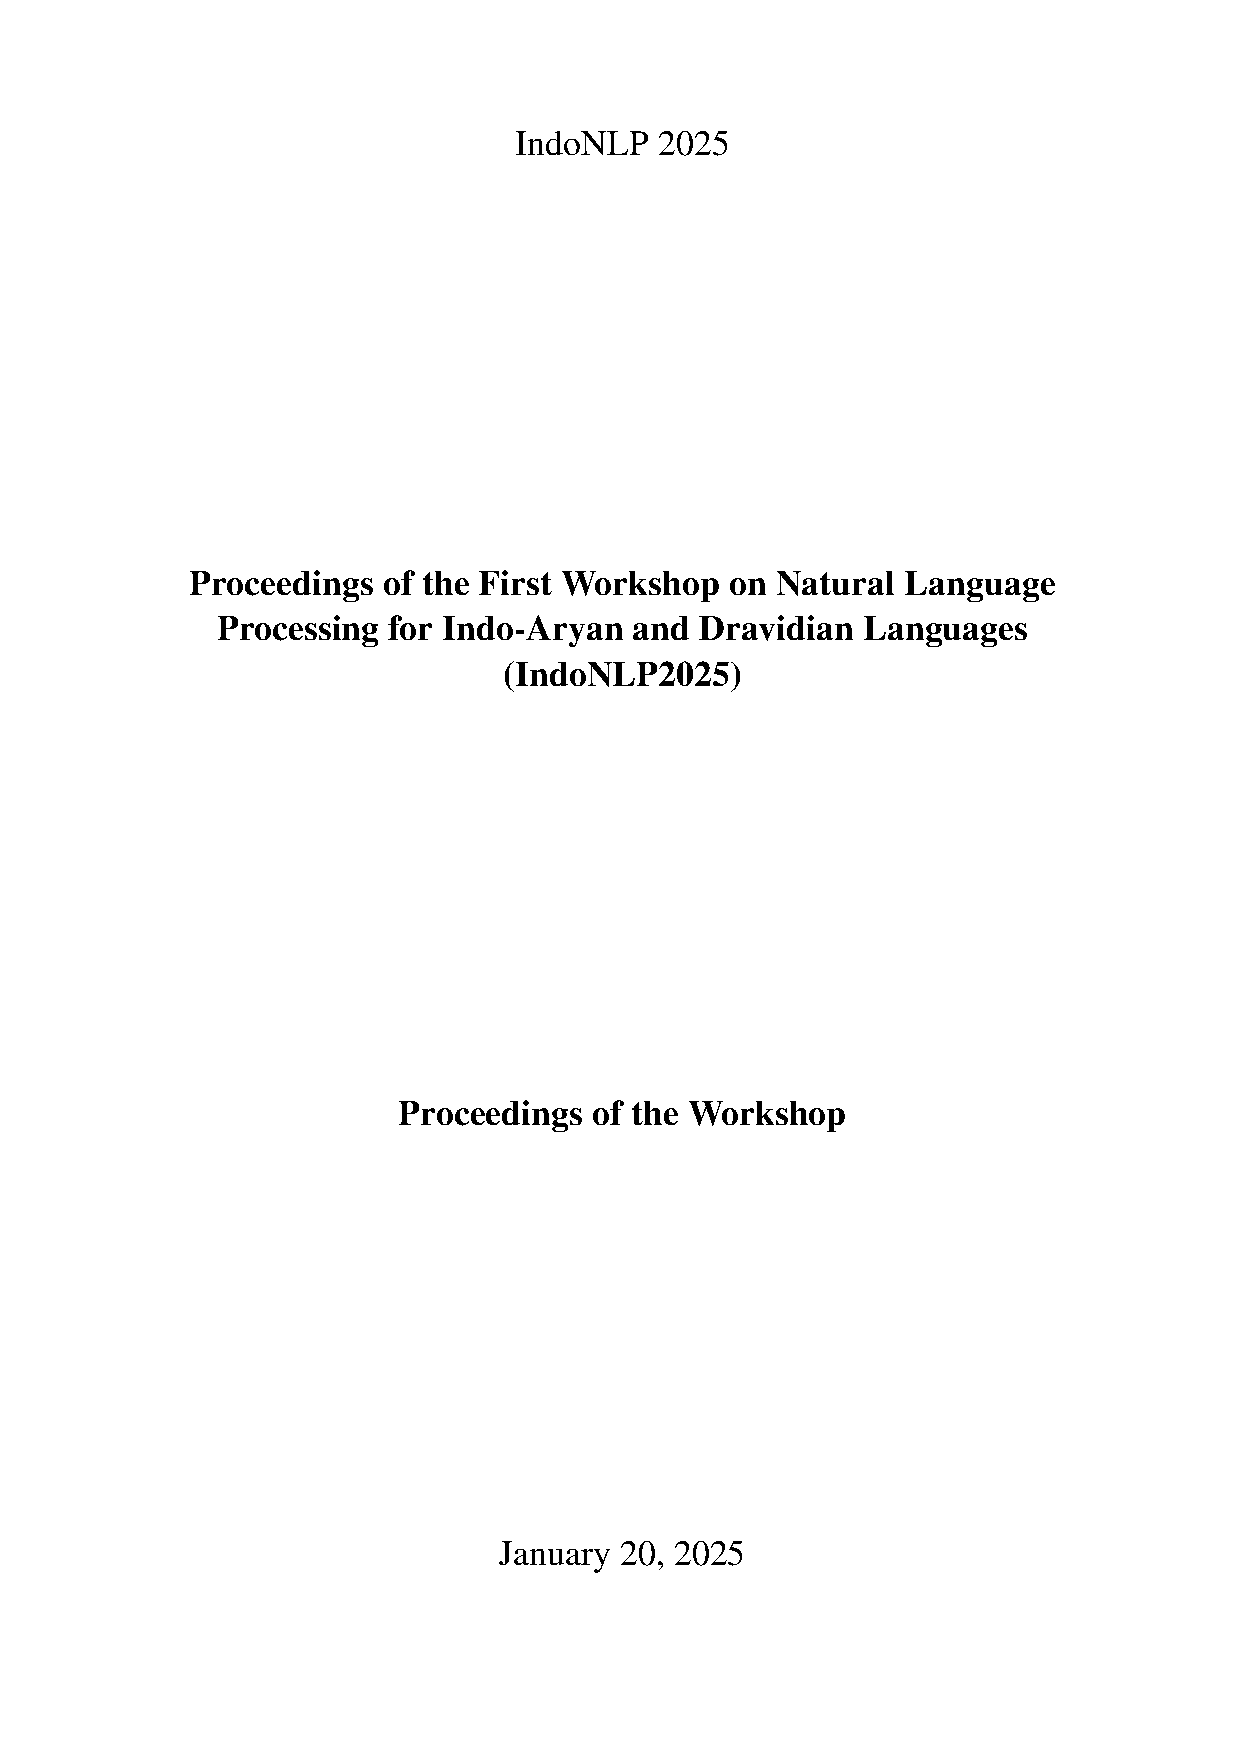
\includepdf{titlepage.pdf}

% -------- FRONT MATTER --------

\includepdfset{pages=-,clip,noautoscale,pagecommand={\thispagestyle{plain}}}

\ifthenelse{\equal{\draftflag}{1}}{\draftframe}{}
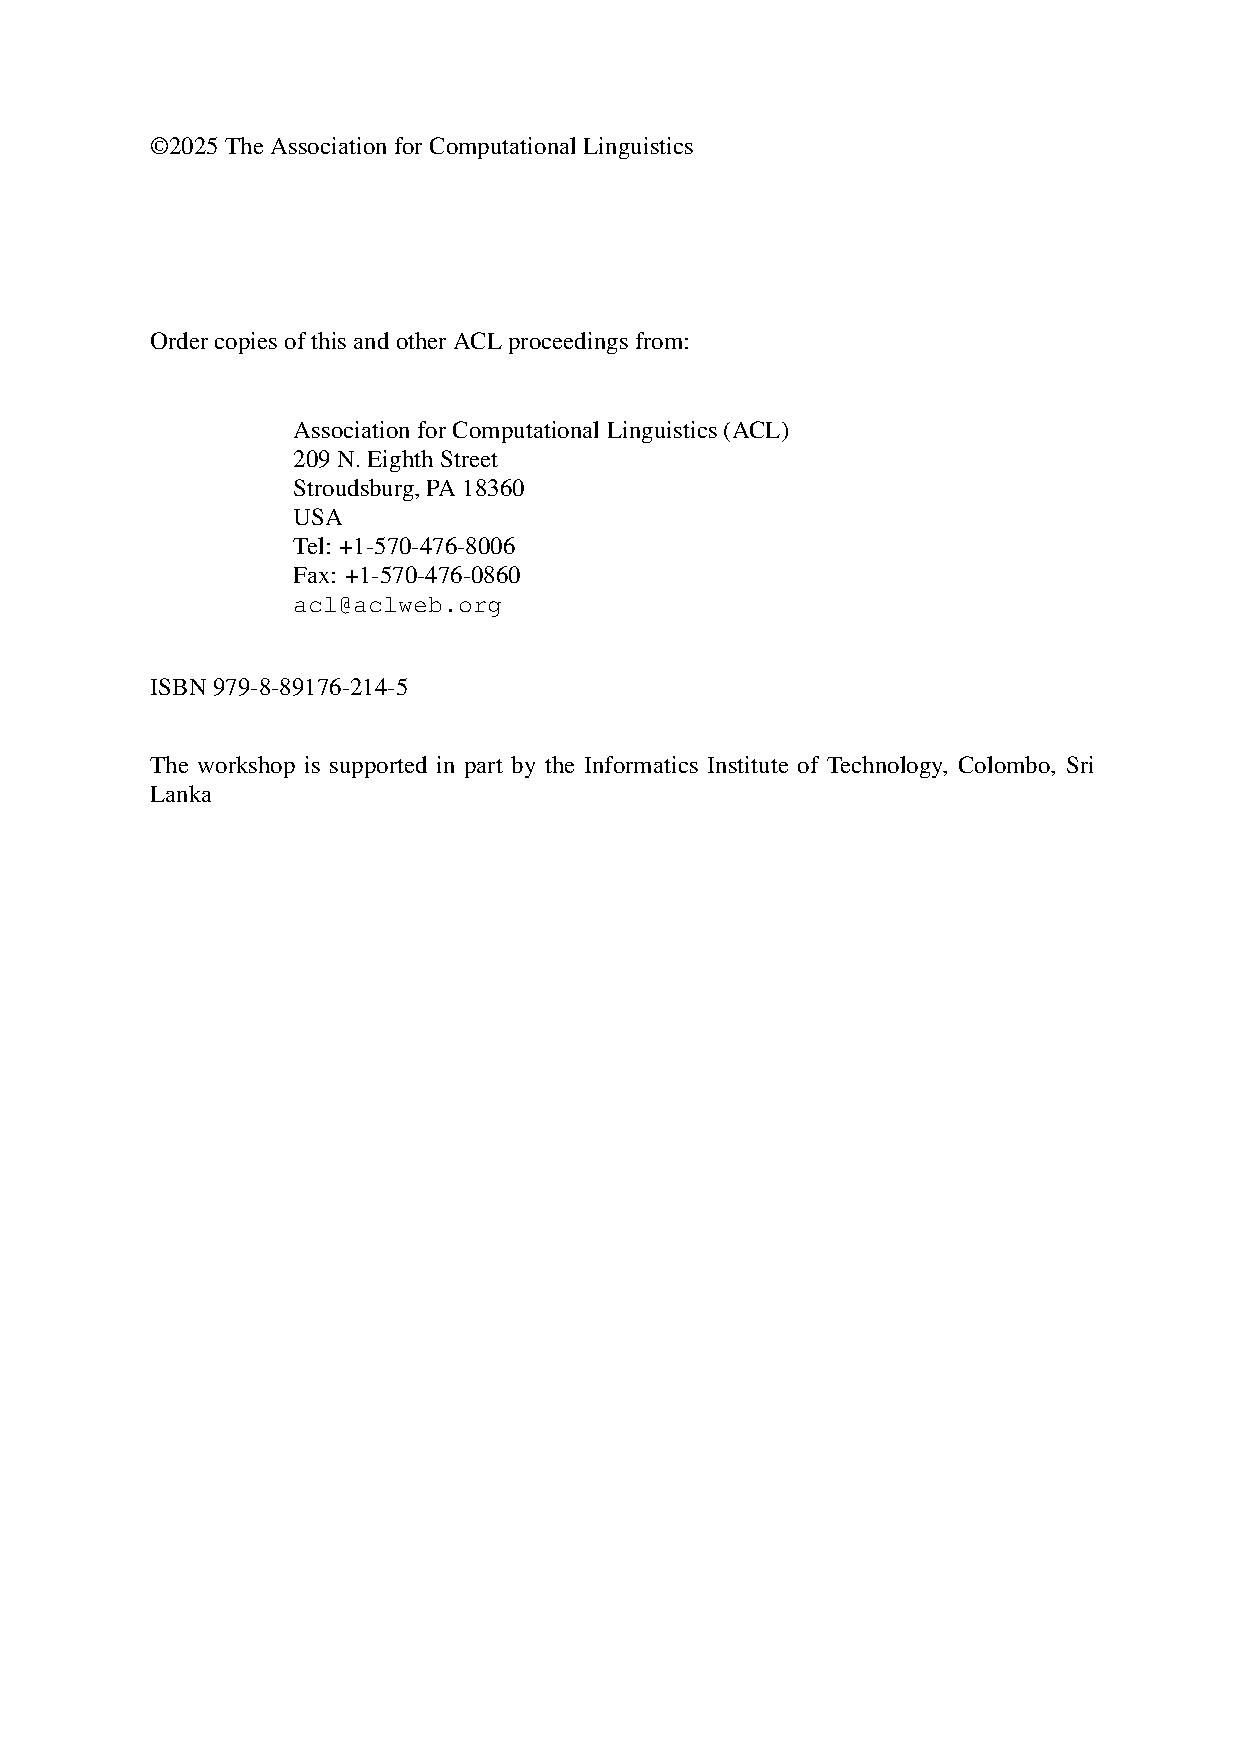
\includepdf{copyright.pdf}

\ifthenelse{\equal{\draftflag}{1}}{\draftframe}{}
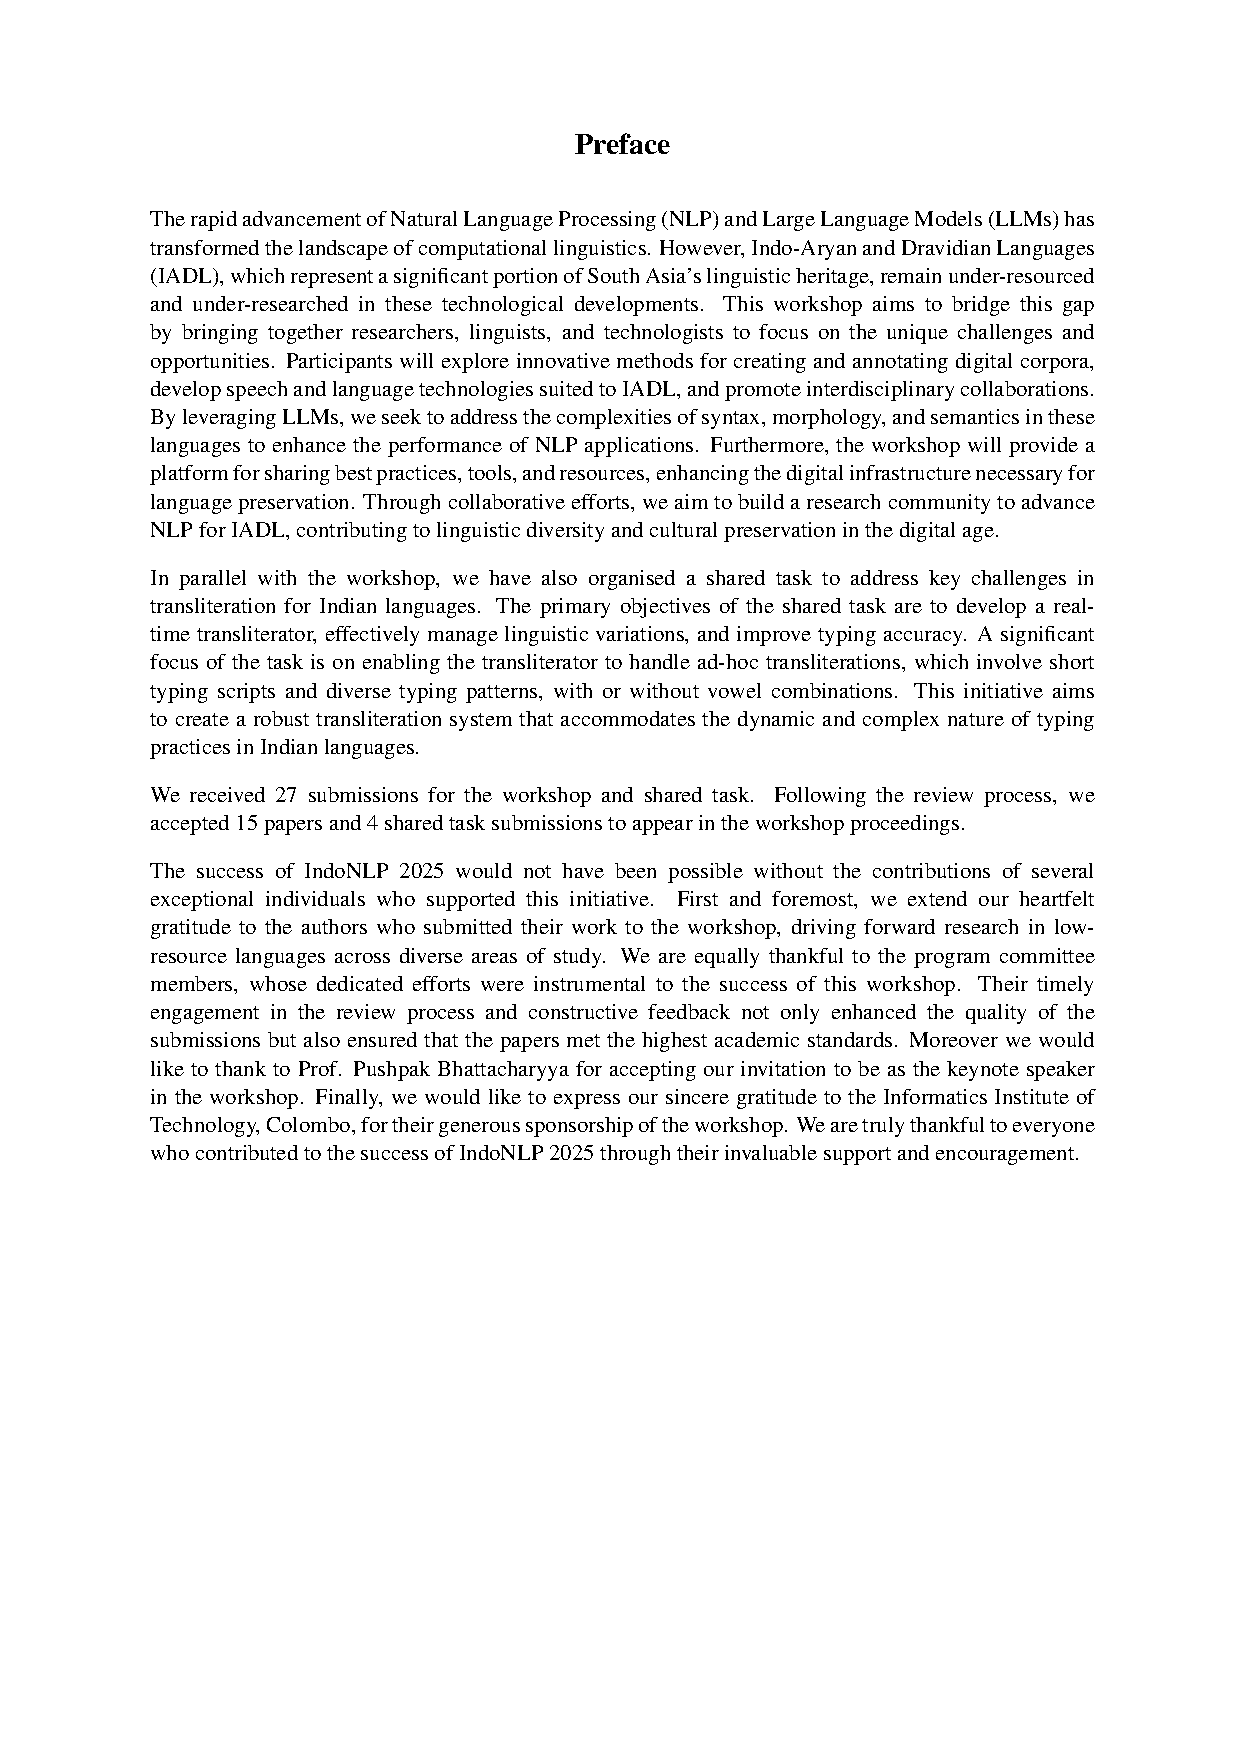
\includepdf{preface.pdf}
\ifthenelse{\isodd{\value{page}}}{}{\newpage \thispagestyle{empty} \phantom{.}}

\ifthenelse{\equal{\draftflag}{1}}{\draftframe}{}
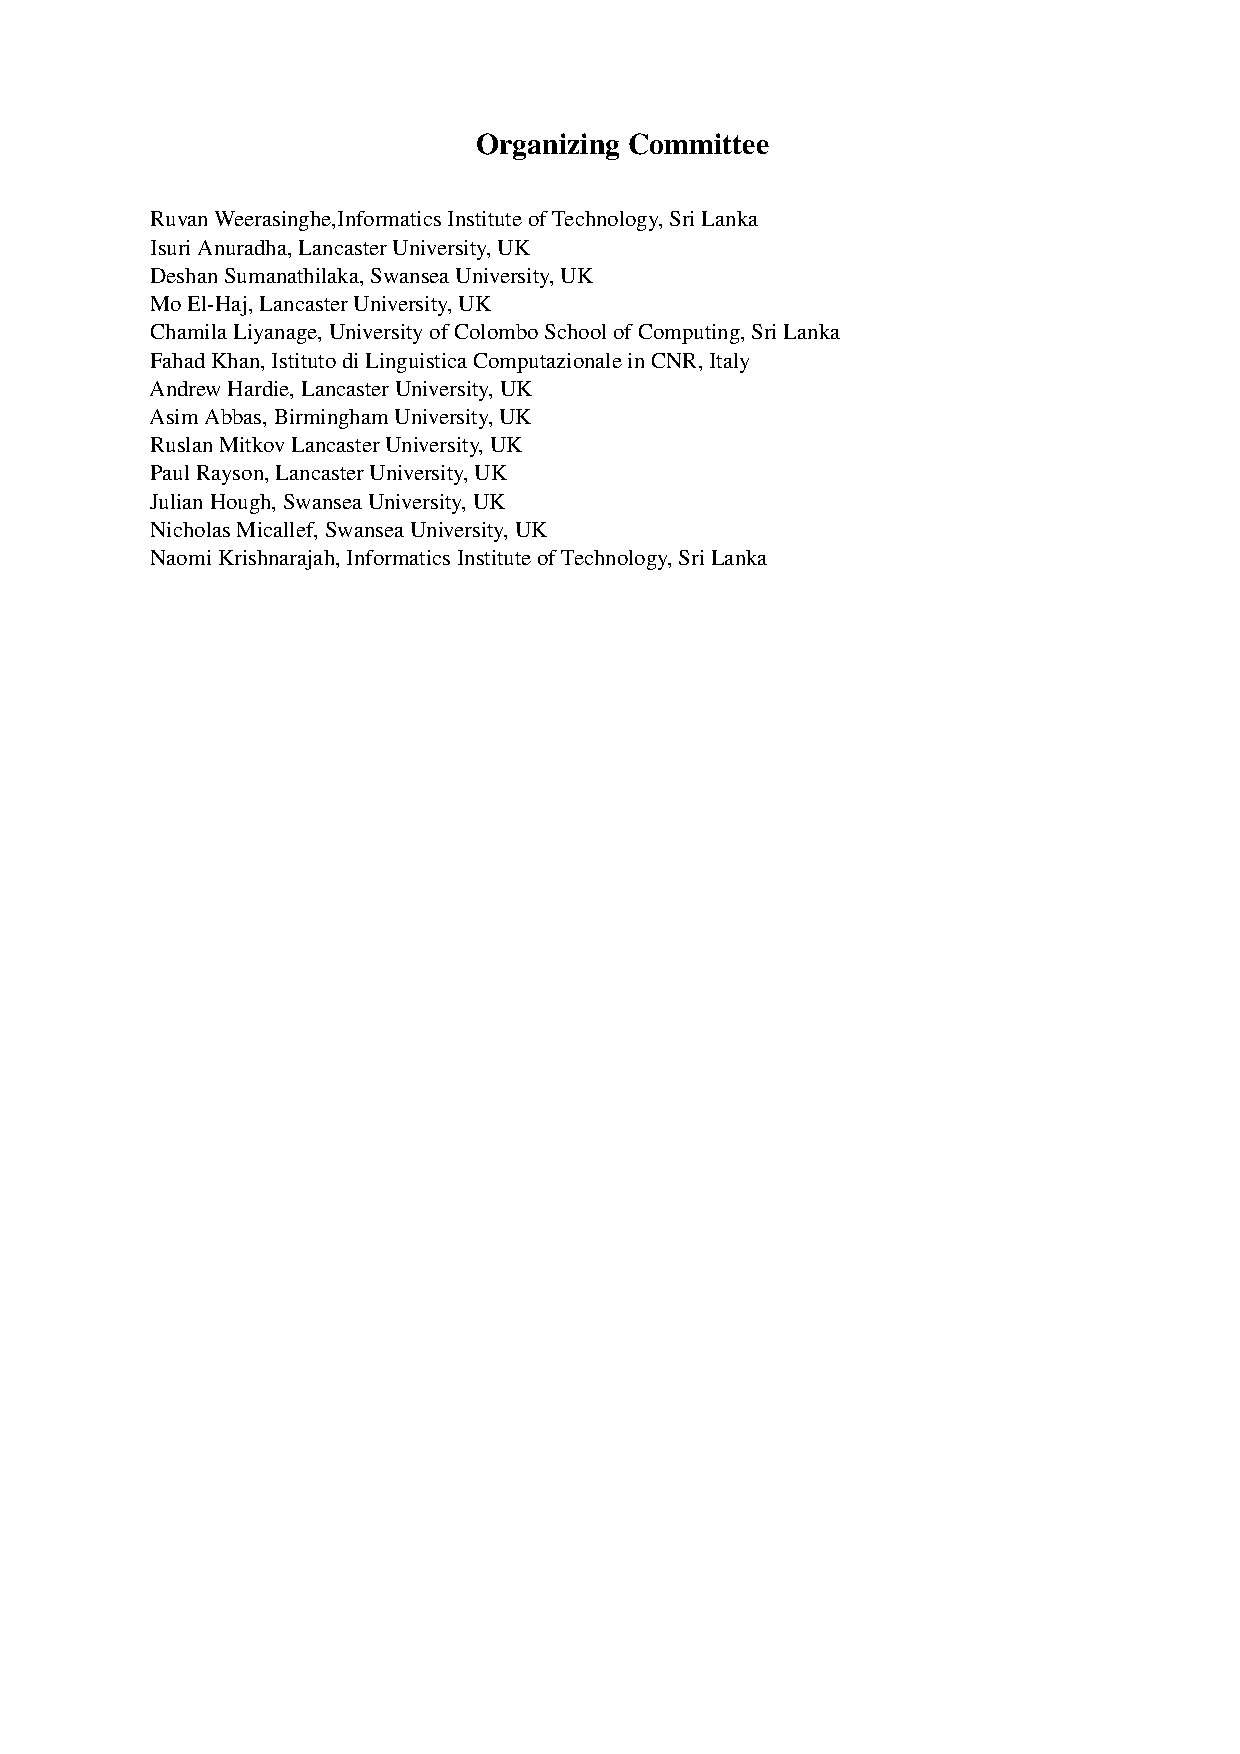
\includepdf{organizers.pdf}
\ifthenelse{\isodd{\value{page}}}{}{\newpage \thispagestyle{empty} \phantom{.}}

\ifthenelse{\equal{\draftflag}{1}}{\draftframe}{}
\setlength{\parindent}{0in}
\setlength{\parskip}{2ex}

\begin{center}
  {\Large \bf Table of Contents}
\end{center}

\vspace*{0.5cm}
\hyperlink{page.1}{\em Crossing Language Boundaries: Evaluation of Large Language Models on Urdu-English Question Answering}\samepage \\
\hspace*{7mm} Samreen kazi, Maria Rahim and Shakeel Ahmed Khoja\dotfill \hyperpage{1}

\hyperlink{page.12}{\em Hindi Reading Comprehension: Do Large Language Models Exhibit Semantic Understanding?}\samepage \\
\hspace*{7mm} Daisy Monika Lal, Paul Rayson and Mo El-Haj\dotfill \hyperpage{12}

\hyperlink{page.23}{\em Machine Translation and Transliteration for Indo-Aryan Languages: A Systematic Review}\samepage \\
\hspace*{7mm} Sandun Sameera Perera and Deshan Koshala Sumanathilaka\dotfill \hyperpage{23}

\hyperlink{page.34}{\em Investigating the Effect of Backtranslation for Indic Languages}\samepage \\
\hspace*{7mm} Sudhansu Bala Das, Samujjal Choudhury, Dr Tapas Kumar Mishra and Dr Bidyut Kr Patra\dotfill \hyperpage{34}

\hyperlink{page.49}{\em BERTopic for Topic Modeling of Hindi Short Texts: A Comparative Study}\samepage \\
\hspace*{7mm} Atharva Mutsaddi, Anvi Jamkhande, Aryan Shirish Thakre and Yashodhara Haribhakta\dotfill \hyperpage{49}

\hyperlink{page.60}{\em Evaluating Structural and Linguistic Quality in Urdu DRS Parsing and Generation through Bidirectional Evaluation}\samepage \\
\hspace*{7mm} Muhammad Saad Amin, Luca Anselma and Alessandro Mazzei\dotfill \hyperpage{60}

\hyperlink{page.71}{\em Studying the Effect of Hindi Tokenizer Performance on Downstream Tasks}\samepage \\
\hspace*{7mm} Rashi Goel and Fatiha Sadat\dotfill \hyperpage{71}

\hyperlink{page.77}{\em Adapting Multilingual LLMs to Low-Resource Languages using Continued Pre-training and Synthetic Corpus: A Case Study for Hindi LLMs}\samepage \\
\hspace*{7mm} Raviraj Joshi, Kanishk Singla, Anusha Kamath, Raunak Kalani, Rakesh Paul, Utkarsh Vaidya, Sanjay Singh Chauhan, Niranjan Wartikar and Eileen Long\dotfill \hyperpage{77}

\hyperlink{page.85}{\em OVQA: A Dataset for Visual Question Answering and Multimodal Research in Odia Language}\samepage \\
\hspace*{7mm} Shantipriya Parida, Shashikanta Sahoo, Sambit Sekhar, Kalyanamalini Sahoo, Ketan Kotwal, Sonal Khosla, Satya Ranjan Dash, Aneesh Bose, Guneet Singh Kohli, Smruti Smita Lenka and Ondřej Bojar\dotfill \hyperpage{85}

\hyperlink{page.93}{\em Advancing Multilingual Speaker Identification and Verification for Indo-Aryan and Dravidian Languages}\samepage \\
\hspace*{7mm} Braveenan Sritharan and Uthayasanker Thayasivam\dotfill \hyperpage{93}

\hyperlink{page.100}{\em Sentiment Analysis of Sinhala News Comments Using Transformers}\samepage \\
\hspace*{7mm} Isuru Bandaranayake and Hakim Usoof\dotfill \hyperpage{100}

\hyperlink{page.109}{\em ExMute: A Context-Enriched Multimodal Dataset for Hateful Memes}\samepage \\
\hspace*{7mm} Riddhiman Swanan Debnath, Nahian Beente Firuj, Abdul Wadud Shakib, Sadia Sultana and Md Saiful Islam\dotfill \hyperpage{109}

\hyperlink{page.116}{\em Studying the capabilities of Large Language Models in solving Combinatorics Problems posed in Hindi}\samepage \\
\hspace*{7mm} Yash Kumar and Subhajit Roy\dotfill \hyperpage{116}

\hyperlink{page.126}{\em From Scarcity to Capability: Empowering Fake News Detection in Low-Resource Languages with LLMs}\samepage \\
\hspace*{7mm} Hrithik Majumdar Shibu, Shrestha Datta, Md. Sumon Miah, Nasrullah Sami, Mahruba Sharmin Chowdhury and Md Saiful Islam\dotfill \hyperpage{126}

\hyperlink{page.134}{\em Enhancing Participatory Development Research in South Asia through LLM Agents System: An Empirically-Grounded Methodological Initiative from Field Evidence in Sri Lankan}\samepage \\
\hspace*{7mm} Xinjie Zhao, Hao Wang, Shyaman Maduranga Sriwarnasinghe, Jiacheng Tang, Shiyun Wang, Sayaka Sugiyama and So Morikawa\dotfill \hyperpage{134}

\hyperlink{page.148}{\em Identifying Aggression and Offensive Language in Code-Mixed Tweets: A Multi-Task Transfer Learning Approach}\samepage \\
\hspace*{7mm} Bharath Kancharla, Prabhjot Singh, Lohith Bhagavan Kancharla, Yashita Chama and Raksha Sharma\dotfill \hyperpage{148}

\hyperlink{page.155}{\em Team IndiDataMiner at IndoNLP 2025: Hindi Back Transliteration - Roman to Devanagari using LLaMa}\samepage \\
\hspace*{7mm} Saurabh Kumar, Dhruvkumar Babubhai Kakadiya and Sanasam Ranbir Singh\dotfill \hyperpage{155}

\hyperlink{page.161}{\em IndoNLP 2025 Shared Task: Romanized Sinhala to Sinhala Reverse Transliteration Using BERT}\samepage \\
\hspace*{7mm} Sandun Sameera Perera, Lahiru Prabhath Jayakodi, Deshan Koshala Sumanathilaka and Isuri Anuradha\dotfill \hyperpage{161}

\hyperlink{page.168}{\em Sinhala Transliteration: A Comparative Analysis Between Rule-based and Seq2Seq Approaches}\samepage \\
\hspace*{7mm} Widanalage Mario Yomal De Mel, Kasun Imesha Wickramasinghe, Nisansa de Silva and Surangika Dayani Ranathunga\dotfill \hyperpage{168}

\hyperlink{page.177}{\em Romanized to Native Malayalam Script Transliteration Using an Encoder-Decoder Framework}\samepage \\
\hspace*{7mm} Bajiyo Baiju, Kavya Manohar, Leena G. Pillai and Elizabeth Sherly\dotfill \hyperpage{177}


\ifthenelse{\isodd{\value{page}}}{}{\newpage \thispagestyle{empty} \phantom{.}}

\ifthenelse{\equal{\draftflag}{1}}{\draftframe}{}
\addcontentsline{toc}{chapter}{Program}
\setlength{\parindent}{0in}
\setlength{\parskip}{2ex}
\renewcommand{\baselinestretch}{0.87}

\begin{center}
{\Large \bf
  Conference Program
}
\end{center}
\vspace{3mm}
\begin{tabular}{p{20mm}p{128mm}}
\\{\bf 8.45--9.00} & {\bf Opening Remark} \\
\\
\\{\bf 9.00--10.00} & {\bf Keynote Speech} \\
\\
\\ & {\bf Theme: Language Processing and Evaluation} \\
\\
10.00--10.15 & \hyperlink{page.1}{\em Crossing Language Boundaries: Evaluation of Large Language Models on Urdu-English Question Answering}\\
         & Samreen kazi, Maria Rahim and Shakeel Ahmed Khoja \\
\\

10.15--10.30 & \hyperlink{page.12}{\em Hindi Reading Comprehension: Do Large Language Models Exhibit Semantic Understanding?}\\
         & Daisy Monika Lal, Paul Rayson and Mo El-Haj \\
\\

\\ & {\bf Coffee Break} \\
\\
11.00--11.15 & \hyperlink{page.23}{\em Machine Translation and Transliteration for Indo-Aryan Languages: A Systematic Review}\\
         & Sandun Sameera Perera and Deshan Koshala Sumanathilaka \\
\\

11.15--11.30 & \hyperlink{page.34}{\em Investigating the Effect of Backtranslation for Indic Languages}\\
         & Sudhansu Bala Das, Samujjal Choudhury, Dr Tapas Kumar Mishra and Dr Bidyut Kr Patra \\
\\

11.30--11.45 & \hyperlink{page.49}{\em BERTopic for Topic Modeling of Hindi Short Texts: A Comparative Study}\\
         & Atharva Mutsaddi, Anvi Jamkhande, Aryan Shirish Thakre and Yashodhara Haribhakta \\
\\

11.45--12.00 & \hyperlink{page.60}{\em Evaluating Structural and Linguistic Quality in Urdu DRS Parsing and Generation through Bidirectional Evaluation}\\
         & Muhammad Saad Amin, Luca Anselma and Alessandro Mazzei \\
\\

12.00--12.15 & \hyperlink{page.71}{\em Studying the Effect of Hindi Tokenizer Performance on Downstream Tasks}\\
         & Rashi Goel and Fatiha Sadat \\
\\

12.15--12.30 & \hyperlink{page.77}{\em Adapting Multilingual LLMs to Low-Resource Languages using Continued Pre-training and Synthetic Corpus: A Case Study for Hindi LLMs}\\
         & Raviraj Joshi, Kanishk Singla, Anusha Kamath, Raunak Kalani, Rakesh Paul, Utkarsh Vaidya, Sanjay Singh Chauhan, Niranjan Wartikar and Eileen Long \\
\\

\end{tabular}
\newpage
\begin{tabular}{p{20mm}p{128mm}}
\\
12.30--12.45 & \hyperlink{page.85}{\em OVQA: A Dataset for Visual Question Answering and Multimodal Research in Odia Language}\\
         & Shantipriya Parida, Shashikanta Sahoo, Sambit Sekhar, Kalyanamalini Sahoo, Ketan Kotwal, Sonal Khosla, Satya Ranjan Dash, Aneesh Bose, Guneet Singh Kohli, Smruti Smita Lenka and Ondřej Bojar \\
\\

12.45--13.00 & \hyperlink{page.93}{\em Advancing Multilingual Speaker Identification and Verification for Indo-Aryan and Dravidian Languages}\\
         & Braveenan Sritharan and Uthayasanker Thayasivam \\
\\

\\{\bf 13.00--14.00} & {\bf Lunch Break} \\
\\
\\ & {\bf Theme: Applications and Societal Impact: Applying NLP to Real-World Problems and Societal Challenges} \\
\\
14.00--14.15 & \hyperlink{page.100}{\em Sentiment Analysis of Sinhala News Comments Using Transformers}\\
         & Isuru Bandaranayake and Hakim Usoof \\
\\

14.15--14.30 & \hyperlink{page.109}{\em ExMute: A Context-Enriched Multimodal Dataset for Hateful Memes}\\
         & Riddhiman Swanan Debnath, Nahian Beente Firuj, Abdul Wadud Shakib, Sadia Sultana and Md Saiful Islam \\
\\

14.30--14.45 & \hyperlink{page.116}{\em Studying the capabilities of Large Language Models in solving Combinatorics Problems posed in Hindi}\\
         & Yash Kumar and Subhajit Roy \\
\\

14.45--15.00 & \hyperlink{page.126}{\em From Scarcity to Capability: Empowering Fake News Detection in Low-Resource Languages with LLMs}\\
         & Hrithik Majumdar Shibu, Shrestha Datta, Md. Sumon Miah, Nasrullah Sami, Mahruba Sharmin Chowdhury and Md Saiful Islam \\
\\

15.00--15.15 & \hyperlink{page.134}{\em Enhancing Participatory Development Research in South Asia through LLM Agents System: An Empirically-Grounded Methodological Initiative from Field Evidence in Sri Lankan}\\
         & Xinjie Zhao, Hao Wang, Shyaman Maduranga Sriwarnasinghe, Jiacheng Tang, Shiyun Wang, Sayaka Sugiyama and So Morikawa \\
\\

15.15--15.30 & \hyperlink{page.148}{\em Identifying Aggression and Offensive Language in Code-Mixed Tweets: A Multi-Task Transfer Learning Approach}\\
         & Bharath Kancharla, Prabhjot Singh, Lohith Bhagavan Kancharla, Yashita Chama and Raksha Sharma \\
\\

\end{tabular}
\newpage
\begin{tabular}{p{20mm}p{128mm}}
\\
\\{\bf 15.30--16.00} & {\bf Coffee Break} \\
\\
\\ & {\bf Shared Task Discussion} \\
\\
 & \hyperlink{page.155}{\em Team IndiDataMiner at IndoNLP 2025: Hindi Back Transliteration - Roman to Devanagari using LLaMa}\\
         & Saurabh Kumar, Dhruvkumar Babubhai Kakadiya and Sanasam Ranbir Singh \\
\\

 & \hyperlink{page.161}{\em IndoNLP 2025 Shared Task: Romanized Sinhala to Sinhala Reverse Transliteration Using BERT}\\
         & Sandun Sameera Perera, Lahiru Prabhath Jayakodi, Deshan Koshala Sumanathilaka and Isuri Anuradha \\
\\

 & \hyperlink{page.168}{\em Sinhala Transliteration: A Comparative Analysis Between Rule-based and Seq2Seq Approaches}\\
         & Widanalage Mario Yomal De Mel, Kasun Imesha Wickramasinghe, Nisansa de Silva and Surangika Dayani Ranathunga \\
\\

 & \hyperlink{page.177}{\em Romanized to Native Malayalam Script Transliteration Using an Encoder-Decoder Framework}\\
         & Bajiyo Baiju, Kavya Manohar, Leena G. Pillai and Elizabeth Sherly \\
\\

\\ & {\bf Final Remark} \\
\\


\end{tabular}

\ifthenelse{\isodd{\value{page}}}{}{\newpage \thispagestyle{empty} \phantom{.}}

\end{document}